% Graph 06: Network Lifetime vs Initial Node Energy Budget at 100 nodes
% Data at 2.0 J from paper (ADSS=1310s, Trust-RPL=1108s, RPL=1080s);
% remaining protocols and lower energy levels interpolated consistently.
% Include in main document with: % Graph 05: Packet Delivery Ratio vs Traffic Generation Rate at 100 nodes
% Data at 5 pkts/s and 2 pkts/s from paper; other points interpolated consistently.
% Include in main document with: % Graph 04: Normalized Energy Consumption per Delivered Packet vs Number of Nodes
% Data points at 100 nodes from paper; 50 and 200 nodes interpolated consistently.
% Include in main document with: % Graph 03: Average End-to-End Delay vs Number of Deployed Nodes
% Data points at 100 nodes from paper; 50 and 200 nodes interpolated consistently.
% Include in main document with: \input{graphs/graph03_delay_vs_nodes}
\documentclass[tikz,border=4pt]{standalone}
\usepackage{pgfplots}
\pgfplotsset{compat=1.18}

\begin{document}
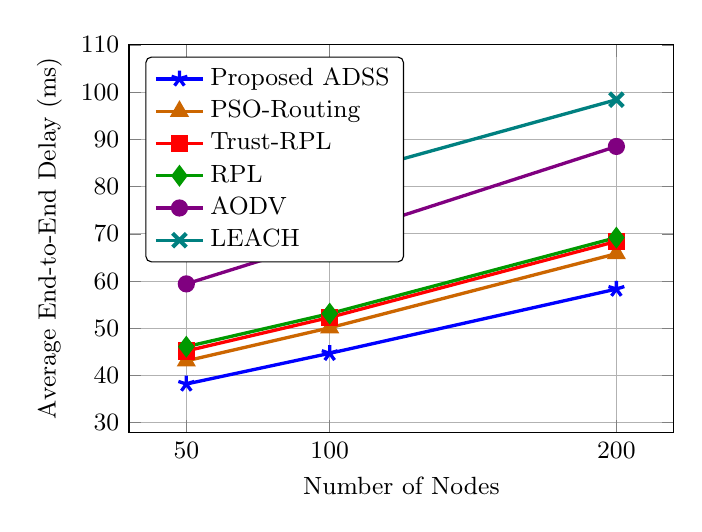
\begin{tikzpicture}
\begin{axis}[
    width=8.5cm,
    height=6.5cm,
    xlabel={Number of Nodes},
    ylabel={Average End-to-End Delay (ms)},
    xmin=30, xmax=220,
    ymin=28, ymax=110,
    xtick={50,100,200},
    xticklabels={50,100,200},
    ytick={30,40,50,60,70,80,90,100,110},
    grid=both,
    grid style={line width=0.2pt, draw=gray!30},
    major grid style={line width=0.4pt, draw=gray!60},
    legend style={
        at={(0.03,0.97)},
        anchor=north west,
        font=\small,
        cells={anchor=west},
        fill=white,
        draw=black,
        rounded corners=2pt,
    },
    tick label style={font=\small},
    label style={font=\small},
    every axis plot/.append style={line width=1.2pt},
]
% Proposed ADSS
\addplot[color=blue, mark=star, mark size=3pt]
    coordinates {(50,38.2) (100,44.7) (200,58.3)};
\addlegendentry{Proposed ADSS}
% PSO-Routing
\addplot[color=orange!80!black, mark=triangle*, mark size=2.8pt]
    coordinates {(50,43.1) (100,50.1) (200,65.8)};
\addlegendentry{PSO-Routing}
% Trust-RPL
\addplot[color=red, mark=square*, mark size=2.5pt]
    coordinates {(50,45.2) (100,52.3) (200,68.4)};
\addlegendentry{Trust-RPL}
% RPL
\addplot[color=green!60!black, mark=diamond*, mark size=3pt]
    coordinates {(50,46.1) (100,53.1) (200,69.2)};
\addlegendentry{RPL}
% AODV
\addplot[color=violet, mark=*, mark size=2.5pt]
    coordinates {(50,59.4) (100,68.9) (200,88.5)};
\addlegendentry{AODV}
% LEACH
\addplot[color=teal, mark=x, mark size=3.5pt, mark options={line width=1.5pt}]
    coordinates {(50,70.2) (100,81.6) (200,98.4)};
\addlegendentry{LEACH}
\end{axis}
\end{tikzpicture}
\end{document}

\documentclass[tikz,border=4pt]{standalone}
\usepackage{pgfplots}
\pgfplotsset{compat=1.18}

\begin{document}
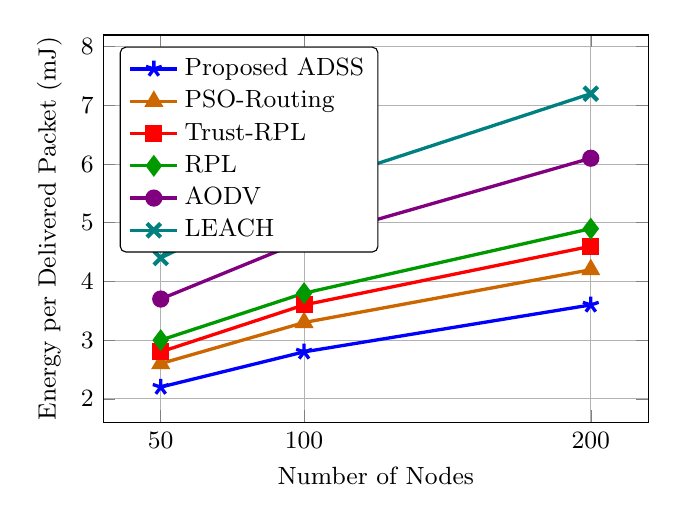
\begin{tikzpicture}
\begin{axis}[
    width=8.5cm,
    height=6.5cm,
    xlabel={Number of Nodes},
    ylabel={Energy per Delivered Packet (mJ)},
    xmin=30, xmax=220,
    ymin=1.6, ymax=8.2,
    xtick={50,100,200},
    xticklabels={50,100,200},
    ytick={2,3,4,5,6,7,8},
    grid=both,
    grid style={line width=0.2pt, draw=gray!30},
    major grid style={line width=0.4pt, draw=gray!60},
    legend style={
        at={(0.03,0.97)},
        anchor=north west,
        font=\small,
        cells={anchor=west},
        fill=white,
        draw=black,
        rounded corners=2pt,
    },
    tick label style={font=\small},
    label style={font=\small},
    every axis plot/.append style={line width=1.2pt},
]
% Proposed ADSS
\addplot[color=blue, mark=star, mark size=3pt]
    coordinates {(50,2.2) (100,2.8) (200,3.6)};
\addlegendentry{Proposed ADSS}
% PSO-Routing
\addplot[color=orange!80!black, mark=triangle*, mark size=2.8pt]
    coordinates {(50,2.6) (100,3.3) (200,4.2)};
\addlegendentry{PSO-Routing}
% Trust-RPL
\addplot[color=red, mark=square*, mark size=2.5pt]
    coordinates {(50,2.8) (100,3.6) (200,4.6)};
\addlegendentry{Trust-RPL}
% RPL
\addplot[color=green!60!black, mark=diamond*, mark size=3pt]
    coordinates {(50,3.0) (100,3.8) (200,4.9)};
\addlegendentry{RPL}
% AODV
\addplot[color=violet, mark=*, mark size=2.5pt]
    coordinates {(50,3.7) (100,4.7) (200,6.1)};
\addlegendentry{AODV}
% LEACH
\addplot[color=teal, mark=x, mark size=3.5pt, mark options={line width=1.5pt}]
    coordinates {(50,4.4) (100,5.6) (200,7.2)};
\addlegendentry{LEACH}
\end{axis}
\end{tikzpicture}
\end{document}

\documentclass[tikz,border=4pt]{standalone}
\usepackage{pgfplots}
\pgfplotsset{compat=1.18}

\begin{document}
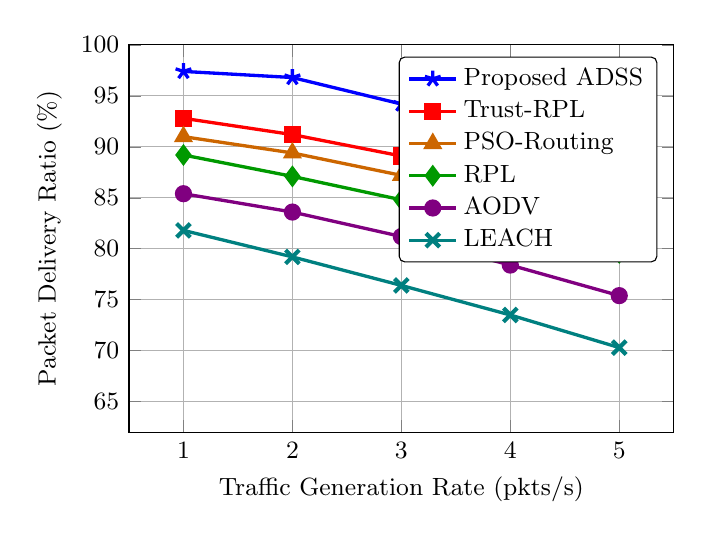
\begin{tikzpicture}
\begin{axis}[
    width=8.5cm,
    height=6.5cm,
    xlabel={Traffic Generation Rate (pkts/s)},
    ylabel={Packet Delivery Ratio (\%)},
    xmin=0.5, xmax=5.5,
    ymin=62, ymax=100,
    xtick={1,2,3,4,5},
    ytick={65,70,75,80,85,90,95,100},
    grid=both,
    grid style={line width=0.2pt, draw=gray!30},
    major grid style={line width=0.4pt, draw=gray!60},
    legend style={
        at={(0.97,0.97)},
        anchor=north east,
        font=\small,
        cells={anchor=west},
        fill=white,
        draw=black,
        rounded corners=2pt,
    },
    tick label style={font=\small},
    label style={font=\small},
    every axis plot/.append style={line width=1.2pt},
]
% Proposed ADSS
\addplot[color=blue, mark=star, mark size=3pt]
    coordinates {(1,97.4) (2,96.8) (3,94.2) (4,91.8) (5,88.2)};
\addlegendentry{Proposed ADSS}
% Trust-RPL
\addplot[color=red, mark=square*, mark size=2.5pt]
    coordinates {(1,92.8) (2,91.2) (3,89.1) (4,87.2) (5,83.9)};
\addlegendentry{Trust-RPL}
% PSO-Routing
\addplot[color=orange!80!black, mark=triangle*, mark size=2.8pt]
    coordinates {(1,91.0) (2,89.4) (3,87.2) (4,84.6) (5,81.3)};
\addlegendentry{PSO-Routing}
% RPL
\addplot[color=green!60!black, mark=diamond*, mark size=3pt]
    coordinates {(1,89.2) (2,87.1) (3,84.8) (4,82.1) (5,79.6)};
\addlegendentry{RPL}
% AODV
\addplot[color=violet, mark=*, mark size=2.5pt]
    coordinates {(1,85.4) (2,83.6) (3,81.2) (4,78.4) (5,75.4)};
\addlegendentry{AODV}
% LEACH
\addplot[color=teal, mark=x, mark size=3.5pt, mark options={line width=1.5pt}]
    coordinates {(1,81.8) (2,79.2) (3,76.4) (4,73.5) (5,70.3)};
\addlegendentry{LEACH}
\end{axis}
\end{tikzpicture}
\end{document}

\documentclass[tikz,border=4pt]{standalone}
\usepackage{pgfplots}
\pgfplotsset{compat=1.18}

\begin{document}
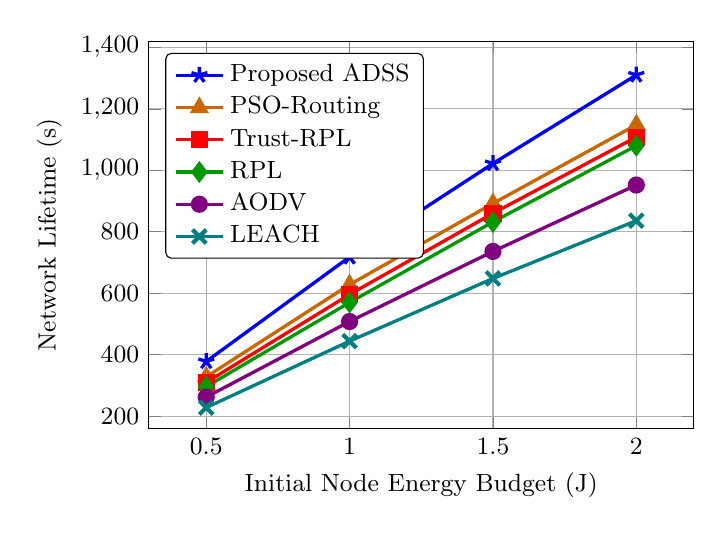
\begin{tikzpicture}
\begin{axis}[
    width=8.5cm,
    height=6.5cm,
    xlabel={Initial Node Energy Budget (J)},
    ylabel={Network Lifetime (s)},
    xmin=0.3, xmax=2.2,
    ymin=160, ymax=1420,
    xtick={0.5,1.0,1.5,2.0},
    ytick={200,400,600,800,1000,1200,1400},
    grid=both,
    grid style={line width=0.2pt, draw=gray!30},
    major grid style={line width=0.4pt, draw=gray!60},
    legend style={
        at={(0.03,0.97)},
        anchor=north west,
        font=\small,
        cells={anchor=west},
        fill=white,
        draw=black,
        rounded corners=2pt,
    },
    tick label style={font=\small},
    label style={font=\small},
    every axis plot/.append style={line width=1.2pt},
]
% Proposed ADSS
\addplot[color=blue, mark=star, mark size=3pt]
    coordinates {(0.5,378) (1.0,718) (1.5,1022) (2.0,1310)};
\addlegendentry{Proposed ADSS}
% PSO-Routing
\addplot[color=orange!80!black, mark=triangle*, mark size=2.8pt]
    coordinates {(0.5,328) (1.0,628) (1.5,892) (2.0,1148)};
\addlegendentry{PSO-Routing}
% Trust-RPL
\addplot[color=red, mark=square*, mark size=2.5pt]
    coordinates {(0.5,310) (1.0,596) (1.5,860) (2.0,1108)};
\addlegendentry{Trust-RPL}
% RPL
\addplot[color=green!60!black, mark=diamond*, mark size=3pt]
    coordinates {(0.5,296) (1.0,570) (1.5,832) (2.0,1080)};
\addlegendentry{RPL}
% AODV
\addplot[color=violet, mark=*, mark size=2.5pt]
    coordinates {(0.5,262) (1.0,508) (1.5,736) (2.0,952)};
\addlegendentry{AODV}
% LEACH
\addplot[color=teal, mark=x, mark size=3.5pt, mark options={line width=1.5pt}]
    coordinates {(0.5,228) (1.0,444) (1.5,648) (2.0,836)};
\addlegendentry{LEACH}
\end{axis}
\end{tikzpicture}
\end{document}
